%% This is emulateapj reformatting of the AASTEX sample document
%%
\documentclass{emulateapj}
\usepackage[colorlinks,urlcolor=blue,citecolor=blue,linkcolor=blue]{hyperref} 
\usepackage{graphicx,natbib}
\citestyle{aa}
\usepackage[space]{grffile}
\usepackage{latexsym}
\usepackage{amsfonts,amsmath,amssymb}
\usepackage{url}
\usepackage[utf8]{inputenc}
\usepackage{fancyref}
\usepackage{hyperref}
\usepackage{multirow}
\hypersetup{colorlinks=false,pdfborder={0 0 0},}

\newcommand{\rf}{\emph{realfast}}
\newcommand{\frb}{\emph{FRB 121102}}

\begin{document}

\title{\frb: Very Large Array Burst Properties and Implications for Overall FRB Population}
\shorttitle{\frb Burst Properties}
\shortauthors{Law et al.}

\author{Casey J. Law\altaffilmark{1}}
\author{Dewey}
\author{Cheetham}
\author{Howe}
\altaffiltext{1}{Dept of Astronomy and Radio Astronomy Lab, Univ. of California, Berkeley, CA}

\begin{abstract}
The highly-dispersed, millisecond radio transients known as Fast Radio Bursts have recently emerged as a new class...

The discovery of repeating bursts from \frb has shown that at least some FRBs are not cataclysmic and opened potential for studying a homogenous sample of bursts...
Our recent coordinated campaign with the Very Large Array and Arecibo Observatory has made the first direct, arcsecond-scale localization of an FRB and unambiguously associated it with counterparts in other observations. This campaign detected nine bursts at the VLA from 2.5 to 3.5~GHz and many more at Arecibo, GBT, and Effelsberg. The coordination of these observations allow us to refine our picture of the physical processes in \frb.

With so many bursts, we can make the first reliable measures of burst flux distribution and temporal statistics...

The connection of \frb to the overall population...

\end{abstract}

\section{Introduction}
Fast Radio Bursts (FRBs) are a new class of millisecond-duration radio transient with a dispersion measure (DM) that implies it originate outside of our Galaxy. At extragalactic (and potentially cosmological) distances, they are not only unusually luminous, but they provide a new tracer of other galaxies and the intergalactic medium (IGM). In this way, FRBs have opened a whole new playground in astrophysics \citep{}. However, that potential has been hamstrung by the lack of a definitive association of an FRB to an extragalactic host.

This paper is part of a series that presents the first localization and host identification of an FRB (CITE, CITE, ...). \frb, also known as the ``repeating FRB'', was first detected in November 2012 by the Arecibo Observatory \citep{2014ApJ...790..101S}. In mid 2015, new Arecibo observations revealed a series of bursts at the same DM and sky position demonstrating that FRBs are capable of repetition \citep{2016Natur.531..202S}. Beginning in August of 2015, we made the first of nine detections of \frb with the Very Large Array (CITE) and localized it with a precision of 0.1\arcsec. Deep radio and optical observing shows that \frb is unambiguously associated with a persistent radio and optical source at a redshift of 0.193 (CITE).

\frb has now been localized three orders of magnitude better than any other FRB and placed at a cosmological distance. Its lookback (luminosity) distance is 746 (972) Mpc \citep{planck15} is orders of magnitude larger than any other millisecond transient. This shows that FRBs:
\begin{itemize}
 \item are extremely luminous, 
 \item have a significant DM contribution from the IGM, and
 \item can be used to probe the IGM and their host galaxy.
\end{itemize}
The promise of the first reported FRB is being realized \citep{2007Sci...318..777L}.

The cosmological distance for \frb could have wide-ranging implications for the FRB population as a whole. However, it has not been demonstrated that \frb is representative of the overall FRB population. In fact, the unambiguous repetition of its bursts is unique among all FRBs \citep{2015MNRAS.454..457P}, so it is natural to ask whether \frb is representative. An important first step is to demonstrate that the properties of \frb are consistent with the significant body of facts for the overall population \citep{2015MNRAS.451.3278M, 2016MPLA...3130013K}. The repeating nature of \frb provides us with several statistical tests we can use to test this connection.

We can also assume that \frb is representative and use it to constrain the physical processes at play in the overall FRB population. Although we now know that FRBs are luminous, it is not yet clear what process generates the radio bursts themselves \citep{2014PhRvD..89j3009K, 2014ApJ...785L..26L, 2016MNRAS.457..232C}. The simultaneous \frb observing campaign with the VLA, Arecibo, Effelsberg, GBT, and AMI gives a more complete picture of the spectral structure of FRBs. FRB repetition also has strong implications for the number of FRB-generating systems in the universe \citep{2016MNRAS.458L..89C}.

Given that FRBs are now known to be useful probes of the IGM, there is strong justification for continuing searches for new detections and localizations. The relatively faint counterpart to \frb argues that direct localization of the radio burst will continue to be the best way to find optical hosts to measure distances. Our multi-telescope constraints on burst spectra, measurement of host properties, burst rate estimates, and other properties will inform new strategies for finding FRBs...

\section{Observations}
\subsection{VLA}

All observations in August and Septmeber were searched in quasi real-time by a prototype version of \rf. \rf\ is a real-time, fast imaging transient search system. The current, prototype runs on existing hardware of the VLA correlator backend, while the future \rf\ will run on a dedicated GPU cluster. The transient search pipeline software is called ``rtpipe''\footnote{See \url{https://github.com/caseyjlaw/rtpipe}} and is mostly written in Python.

Burst detections and localizations were made within hours of data being recorded.

\subsection{Arecibo}

% from the first paper
During the joint Arecibo-VLA campaign, Arecibo observed with the L-wide receiver, which has an observational frequency range of 1.15 to 1.73~GHz and a full width at half maximum beam size of 3.3 arcmin. The PUPPI pulsar backend was used to record total intensity spectra with time and frequency resolutions of 10.24~$\mu$s and 1.5625~MHz, respectively, and full Stokes polarization information. Each frequency channel was coherently dedispersed to 557~\dmu, thereby eliminating intra-channel dispersion smearing. PUPPI covers a total of 800~MHz of bandwidth centred at 1380.78125~MHz, but only $\sim$ 620~MHz of this band is usable due to radio frequency interference and receiver sensitivity roll-off at the band edges.

\subsection{Effelsberg}



\subsection{AMI}



\section{Results}

\subsection{VLA Detections}

Figure \ref{fig:sgram} shows the spectrograms of all nine bursts detected by \rf.

Computational notebooks to reproduce the transient detection and localization can be found at \url{https://github.com/caseyjlaw/FRB121102}. Time cut-out visibility data are available at \url{https://doi.org/10.7910/DVN/TLDKXG}. Original visibility data are available under VLA program codes 16A-459 and 16A-496 and can be downloaded at \url{http://archive.nrao.edu}.


\begin{figure*}[htb]
\begin{center}
 \begin{minipage}{2\columnwidth}
  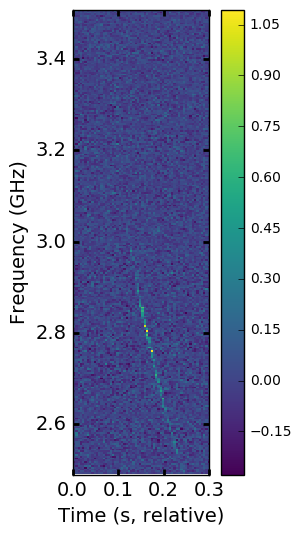
\includegraphics[width=0.25\columnwidth]{sgram_57623.png}
  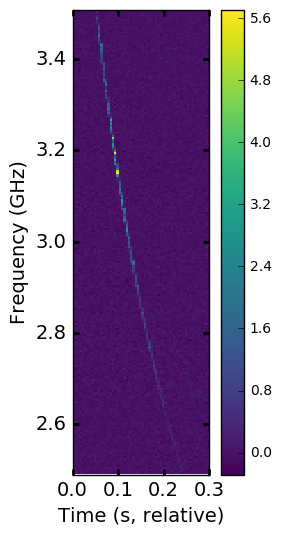
\includegraphics[width=0.25\columnwidth]{sgram_57633_scan7.png}
  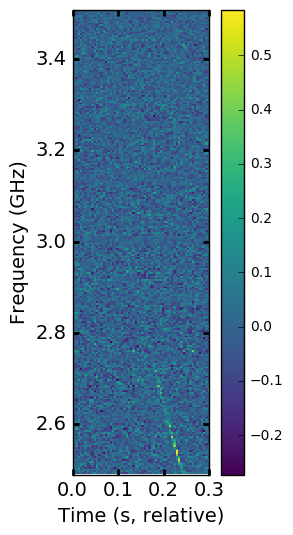
\includegraphics[width=0.25\columnwidth]{sgram_57633_scan13.png}
 \end{minipage}

 \begin{minipage}{2\columnwidth}
  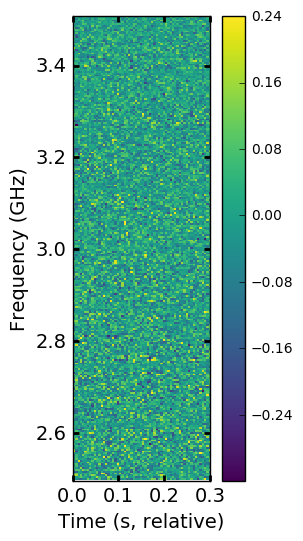
\includegraphics[width=0.25\columnwidth]{sgram_57638.png}
  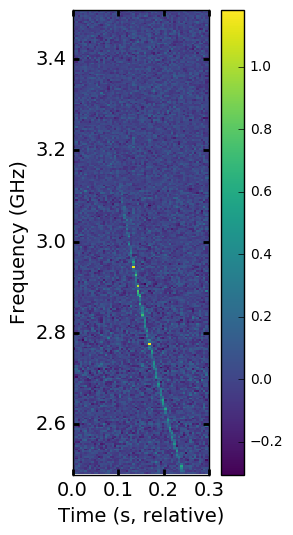
\includegraphics[width=0.25\columnwidth]{sgram_57643.png}
  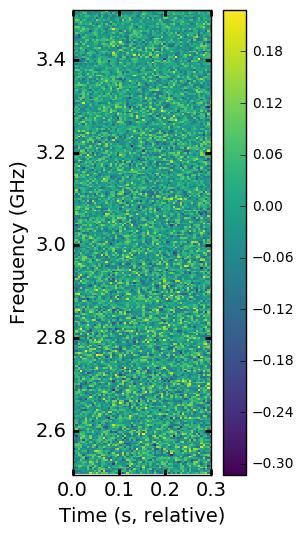
\includegraphics[width=0.25\columnwidth]{sgram_57645.png}
 \end{minipage}

 \begin{minipage}{2\columnwidth}
  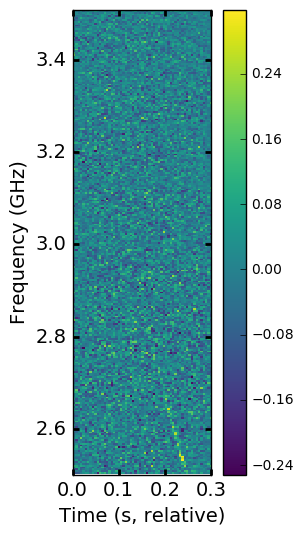
\includegraphics[width=0.25\columnwidth]{sgram_57646.png}
  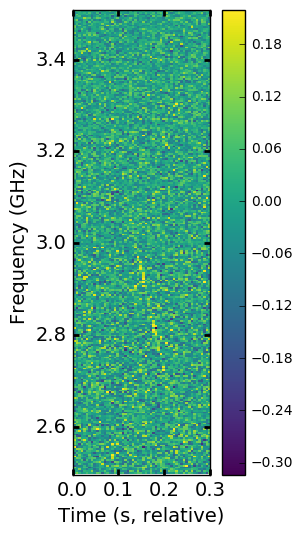
\includegraphics[width=0.25\columnwidth]{sgram_57648.png}
  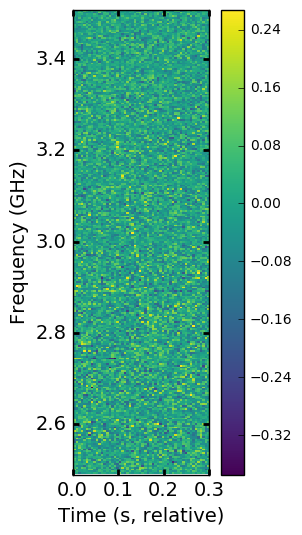
\includegraphics[width=0.25\columnwidth]{sgram_57649.png}
 \end{minipage}
 \caption{Spectrograms (time vs frequency intensity maps) for all nine VLA bursts. Note that bursts are detected in 5~ms images generated from dedispersed visibilities. **NOT SURE WHY ONE FIG LARGER**
 \label{fig:sgram}}
\end{center}
\end{figure*}

\subsection{Multi-Telescope Burst Spectra}

Arecibo had coverage for 57638, 57643, 57645, 57648, and 57649. For 57643 observing was at C band only. At 57648, a burst is seen at 3757s, coincident with the VLA burst.

Effelsberg had simultaneous coverage for bursts on MJD 57648 and 57649. No simultaneous detections.

AMI had simultaneous coverage for bursts on 57643, 57645, 57648, and 57649.

%\begin{table}
%\caption{Caption}
%\centering
%\begin{tabular}{llll}
%\hline
%Field       & RA          & Dec   & Lon. \\ \hline
%\end{tabular}
%\label{fields}
%\end{table} 

\subsection{VLA Spectra}
After detection, we refined the analysis of each burst offline. We used a fine dispersion grid to find the best-fit DM for each burst.

Table?
57623 (DM$=561$ pc cm$^{-3}$)
57633, Scan 7 (DM$=554$ pc cm$^{-3}$)
57633, Scan 13 (DM$=559$ pc cm$^{-3}$)
57638 (DM$=554$ pc cm$^{-3}$)
57643 (DM$=559$ pc cm$^{-3}$)
57645 (DM$=572$ pc cm$^{-3}$)
57646 (DM$=573$ pc cm$^{-3}$)
57648 (DM$=559$ pc cm$^{-3}$)
57649 (DM$=552$ pc cm$^{-3}$).

Dispersion measure changes between bursts significant?

Burst spectra are shown in Figure \ref{fig:spec}...

\begin{figure*}[h!]
\begin{center}
 \begin{minipage}{2\columnwidth}
  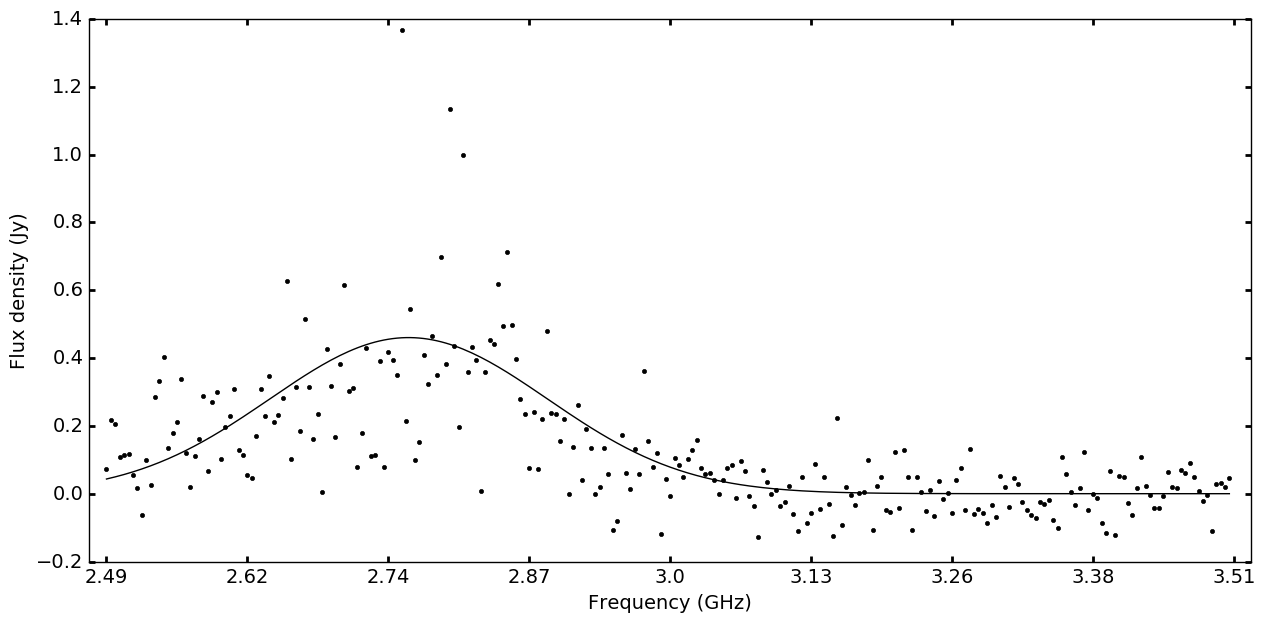
\includegraphics[width=0.3\columnwidth]{spec_57623.png}
  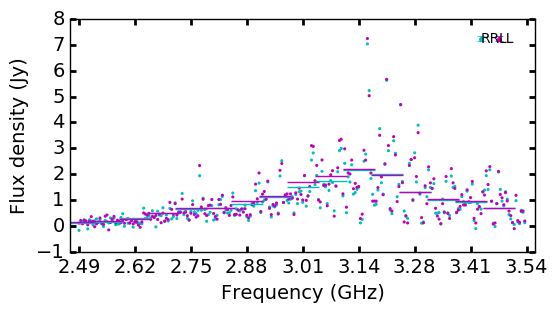
\includegraphics[width=0.3\columnwidth]{spec_57633_scan7.png}
  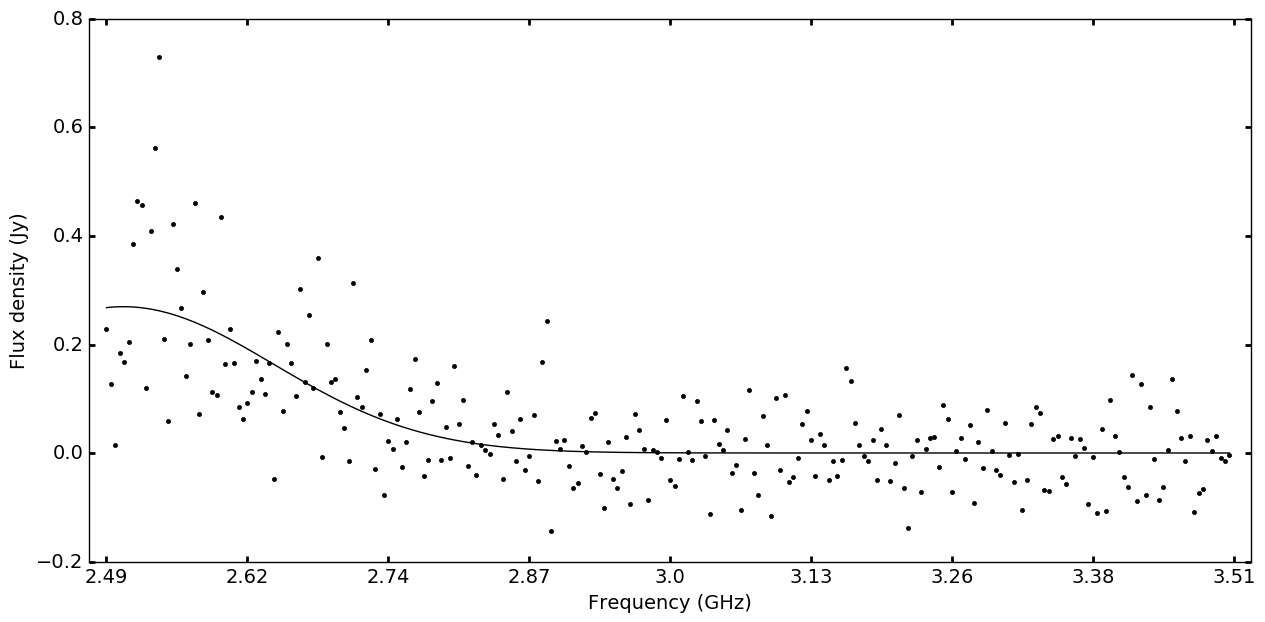
\includegraphics[width=0.3\columnwidth]{spec_57633_scan13.png}
 \end{minipage}

 \begin{minipage}{2\columnwidth}
  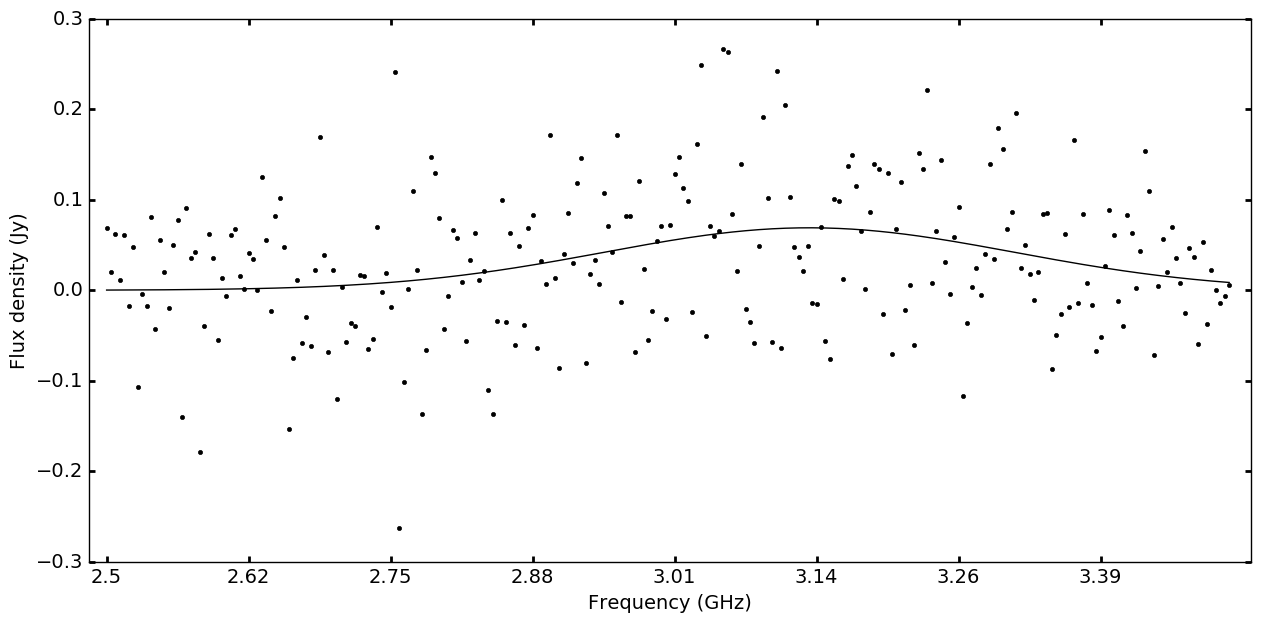
\includegraphics[width=0.3\columnwidth]{spec_57638.png}
  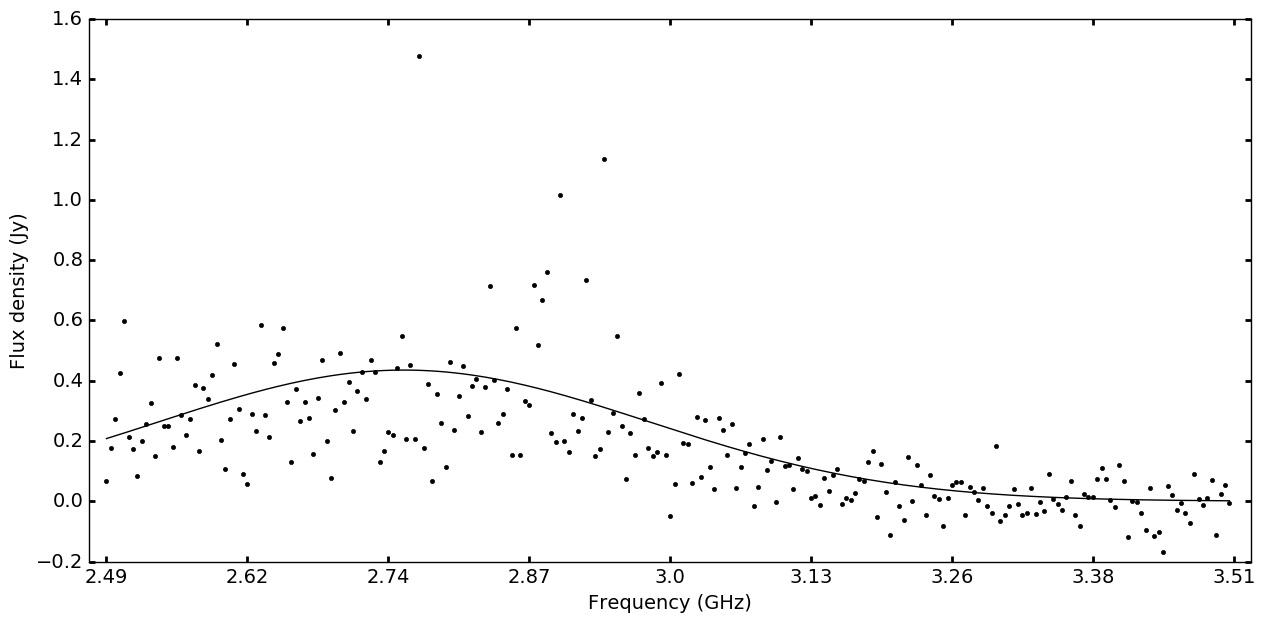
\includegraphics[width=0.3\columnwidth]{spec_57643.png}
  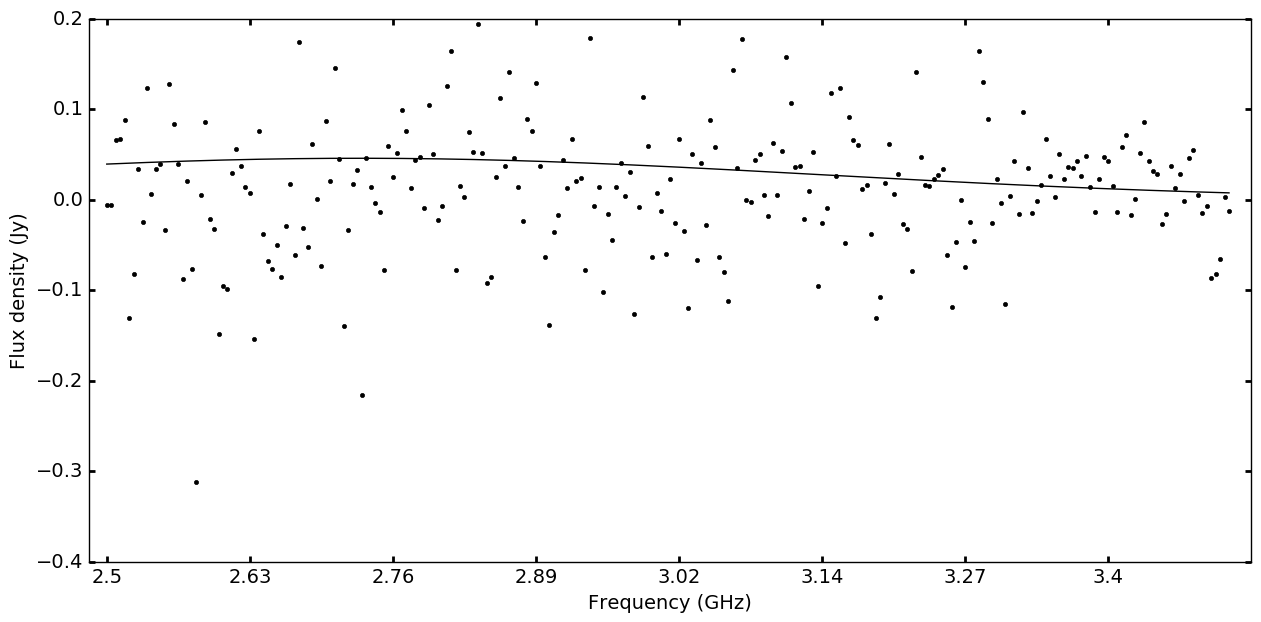
\includegraphics[width=0.3\columnwidth]{spec_57645.png}
 \end{minipage}

 \begin{minipage}{2\columnwidth}
  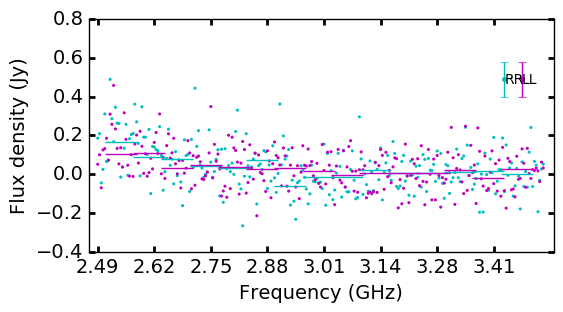
\includegraphics[width=0.3\columnwidth]{spec_57646.png}
  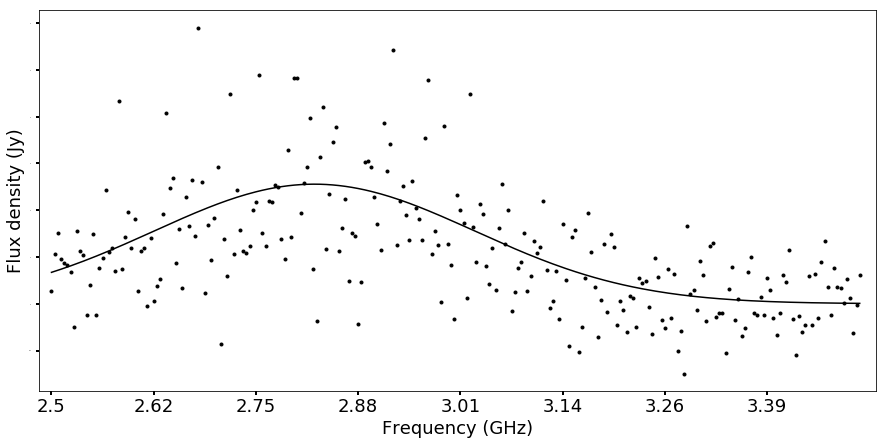
\includegraphics[width=0.3\columnwidth]{spec_57648.png}
  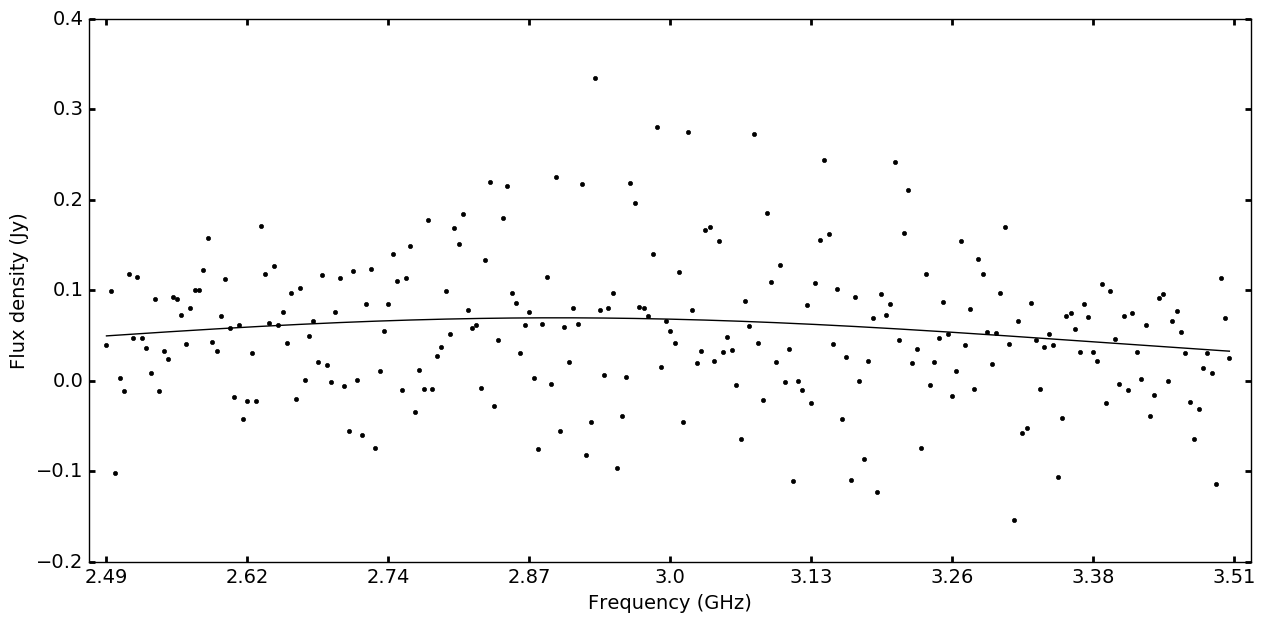
\includegraphics[width=0.3\columnwidth]{spec_57649.png}
 \end{minipage}
\caption{Spectra of nine bursts seen by the VLA from 2.5 to 3.5~GHz.  **LABELS ALL SAME FREQ. SOME SHOULD START HIGHER FOR DROPPED CHANNELS**
 \label{fig:spec}}
\end{center}
\end{figure*}

The VLA S-band recievers natively measure circular polarization, although observations did not include polarization calibration procedures. Crude constraints on circular polarization are possible by comparing the burst intensity in right and left-hand polarized data products. The apparent circular polarization fraction ($(RR-LL)/(RR+LL)$) for the most significant bursts are all less than 3\%. FRB121102 was located 2.3 arcmin away from pointing center, where systematic effects have been measured as large as 3\% (Perley et al 2016, VLA memo). We conclude that the S-band bursts seen by the VLA have a circular polarization of less than 3\%.

\subsection{Brightness Distribution}

The bursts seen by the VLA range in significance from 10 to 150$\sigma$. Offline analysis for flux scale...

Figure \ref{fig:logns} shows the flux distribution of the nine VLA bursts. Flatness...

\begin{figure}[htb]
\begin{center}
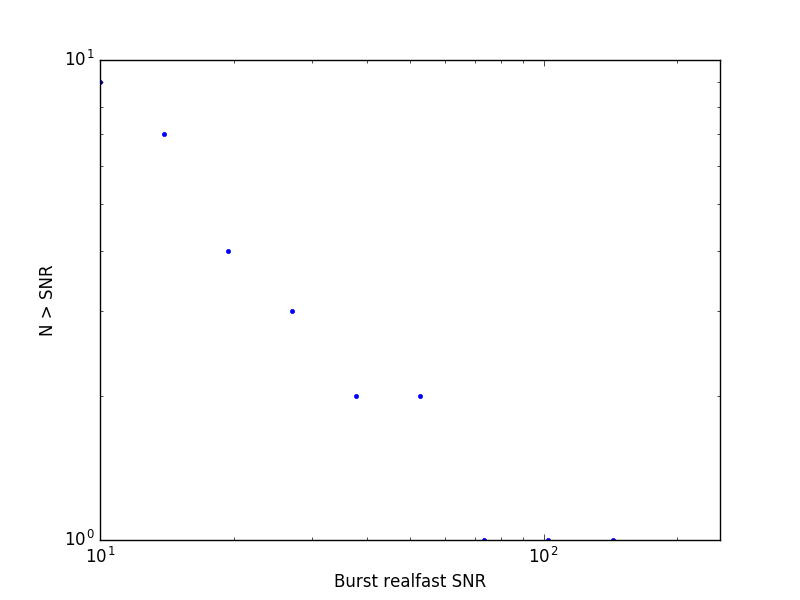
\includegraphics[width=0.9\columnwidth]{logns}
\caption{Log N -- Log SNR distribution of real-time detections of FRB 121102.
\label{fig:logns}}
\end{center}
\end{figure}

Doubts were cast on the first FRB detection (``Lorimer burst'') due to its unusually high brightness. The lack of lower-significance detections suggested that this burst was unlikely to be part of any astrophysical population...

\subsection{Temporal Statistics}
Burst detections were made very inhomogenously though the roughly 60 hours of observing toward FRB 121102. In the first $\sim8$\ hours of observing at L-band and the first $\sim25$\ hours observing at S-band no bursts were detected. Finally, in the last $\sim27$ hours of S-band observing, all nine bursts were detected. Data quality are relatively high and RFI did not significantly impact sensitivity, so the inhomogeneous burst distribution not an observational artifact.

\cite{2016MNRAS.458L..89C}

\begin{figure}[htb]
\begin{center}
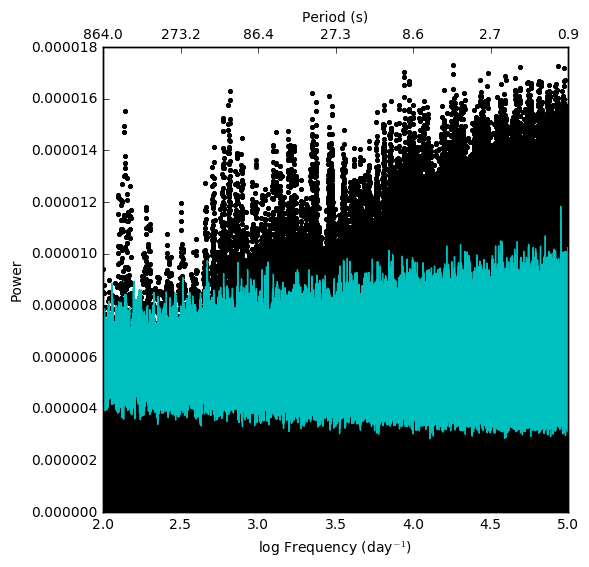
\includegraphics[width=0.9\columnwidth]{lombscargle}
\caption{Lomb-Scargle periodogram.
\label{fig:ls}}
\end{center}
\end{figure}



\section{discussion}

\subsection{Connection to Overall FRB Population}

Flat luminosity distribution of FRB121102 and overall population

Does local (100 Mpc) population with flat luminosity distribution reproduce observed properties? Imagine also how log N/log S cut-offs and scattering biases the intrinsic into the observed distribution (Macquart and Johnston)

Discussion of ``red spectrum'' and Connor \& Pen. Bursts predict bursts therefore repetition constraints of other FRBs are likely weaker than claimed...

Intrinsic versus refractive scintillation

Constraints on repetition assuming "red spectrum" for whole population. Simulation using observed burst temporal statistics...


\subsection{Emission Physics and Burst Energetics}

% from first paper
For a nominal Gpc distance $D$ corresponding to redshifts $z\lesssim 0.3$, the received fluence $A_{\nu}$ from each burst implies  a burst energy
$$E_{\rm burst} = 4\pi D^2 (\delta\Omega/4\pi) A_{\nu} \Delta\nu
\approx 10^{38}\, {\rm erg}\,(\delta\Omega/4\pi) D_{\rm Gpc}^2  (A_{\nu} / 0.1\ {\rm Jy\ ms}) \Delta\nu_{\rm GHz}.$$
The unknown  emission solid angle $\delta\Omega$
could be very small due to relativistic beaming, and together with a distance possibly much smaller than 1~Gpc, could reduce the energy requirement significantly.  However, the {\it total} energy emitted could be larger depending on the duration of the emission in the source frame and other model-dependent details.
Either way, the burst energies from \frb\ are not inconsistent with those that might be expected from the magnetosphere of a compact object\cite{cw16}.

\subsection{Extending FRB 121102 to Other FRBs}

FRB 121102 has a DMhost of xx. Assuming other FRBs have a comparable DMhost, what can we infer about the population as a whole?


\subsection{Observing Strategies}

Targeting known FRBs is optimal

Wide, low-sensitivity searches are best way to conduct a blind search

\section{Conclusions}



\bibliographystyle{apj}

\section*{Acknowledgements}
We thank ...
This project was supported by the University of California Office of the President under Lab Fees Research Program Award 237863. The National Radio Astronomy Observatory is a facility of the National Science Foundation operated under cooperative agreement by Associated Universities, Inc. 

\bibliography{fasttrants.bib}

%\begin{figure}[htb]
%\begin{center}
%\includegraphics[width=0.9\columnwidth]{}
%\caption{
%\label{fig:name}}
%\end{center}
%\end{figure}

%\begin{table}
%\caption{Caption}
%\footnotesize
%\centering
%\begin{tabular}{l|cc|cc|c}
%\hline
%Field       & RA          & Dec   & Lon. & Lat.     & Time \\
%            & \multicolumn{2}{|c|}{(J2000)}  & \multicolumn{2}{|c|}{(Galactic; deg)} & (hrs) \\ \hline
%RA02        & 2:27:53  &  +9:13:24 & 159.0 & --46.8    & 26.25 \\
%PSR J2248-0101 & 22:48:27 & --1:1:48 & 69.3 & --50.6 & 6.5 \\ \hline
%\end{tabular}
%\label{fields}
%\end{table} 

\end{document}

